\question*{
    Design a 4-bit DAC
}

\begin{enumerate}
    \item Setup done.
    \item \textbf{$R_x = 1k \Omega$.} The resistors simply need to be large enough
            to keep the current under the Arduino limits and be lower than the 
            load voltage for Part E.
    \item See \autoref{fig:dacconnected}.
\end{enumerate}

\begin{figure}[ht]
    \centering
    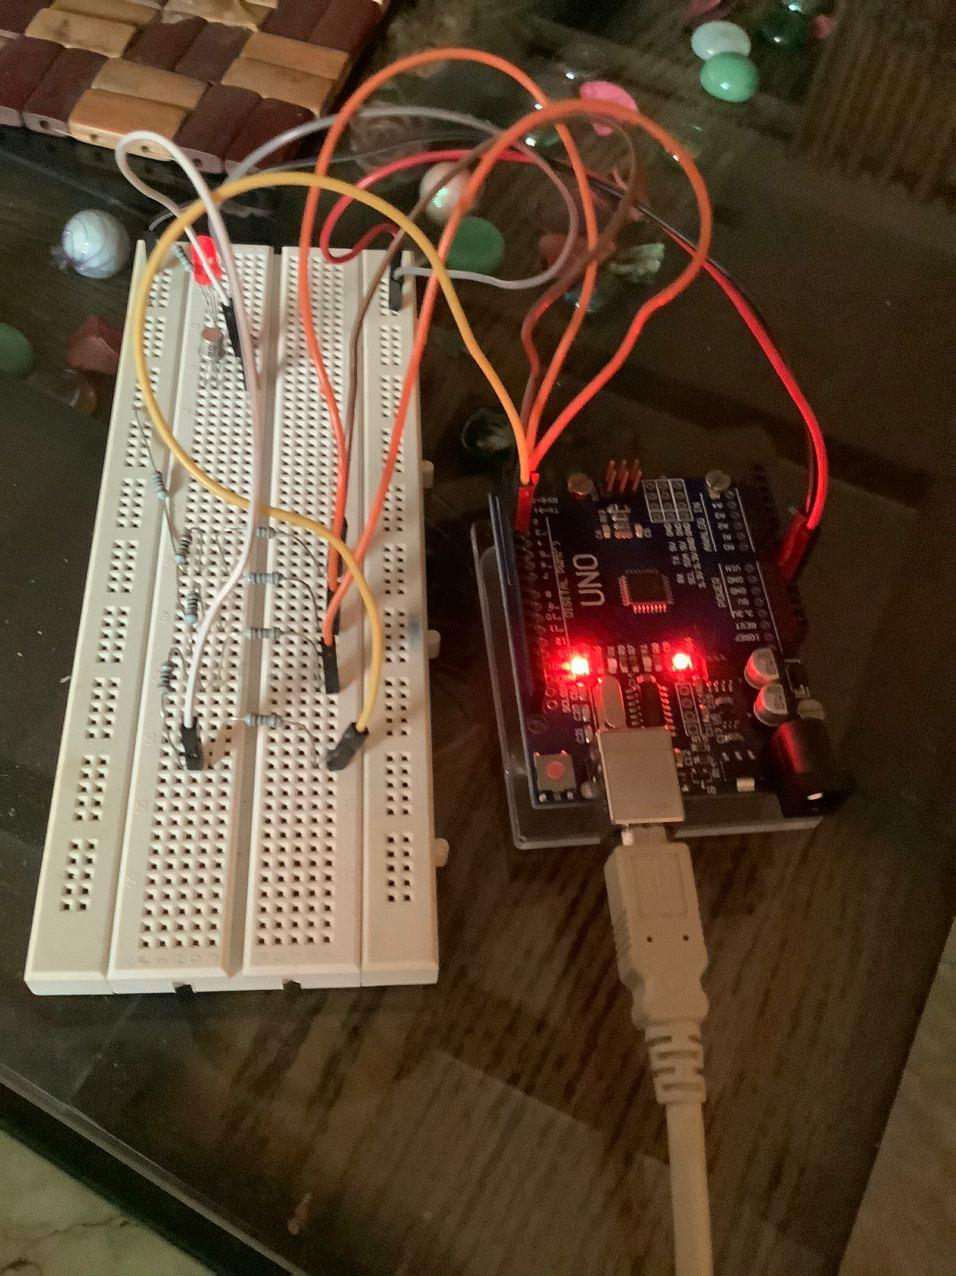
\includegraphics[width=0.4\textwidth]{fig/arduinoconnected-min.jpg}
    \caption{Connected DAC.}
    \label{fig:dacconnected}
\end{figure}